\documentclass[12pt,a4paper]{article}
\usepackage{bold-extra}
\usepackage{appendix}
\usepackage{amsfonts,amsmath,amssymb}
\usepackage{enumerate}
\usepackage{float}
\usepackage{geometry}
\usepackage{graphicx}
\usepackage{latexsym}
\usepackage{listings}
\usepackage{multicol,multirow}
\usepackage{subfigure}
\usepackage{tabularx}
\usepackage{ulem}
\usepackage{tikz}
\usepackage{xcolor}
\geometry{a4paper,left=1in,right=1in,top=1in,bottom=1in}
\begin{document}
\centerline{\Huge{{\textbf{PHYSICS I\ \ Problem Set 5}}}}
\vspace{0.5cm}
\leftline{\large{Name: Haotian Fu}}
\rightline{\large{Student ID: 520021910012}}
\paragraph{\large \textbf{Problem 1}}~{\textbf{Solution}}
\vspace{2mm}\\
\noindent (a) To make the amplitude maximize is to make its denominator minimize since its numerator is a constant. Namely, what we need to ensure is the minimium of
\begin{align}
	(\omega_0^2 - \omega_{\text{dr}}^2)^2 + \left( \frac{b\omega_{\text{dr}}}{m} \right)^2
\end{align}
\par Since equation(1) is equal to
\begin{align}
	\left( \omega_0^2 - \frac{b^2}{2m^2} - \omega_{\text{dr}}^2 \right)^2 + \frac{b^4}{4m^4}
\end{align}
\par we can easily conclude that when
\begin{align}
	\omega_{\text{dr}} = \sqrt{\omega_0^2 - b^2/2m^2}
\end{align}
\par the amplitude is at its maximium. Namely
\begin{align}
	\omega_{\text{res}} = \sqrt{\omega_0^2 - b^2/2m^2}
\end{align}

\noindent (b) we rearrange the formula provided by Problem 1
\begin{align}
	A(\omega_{\text{dr}}) &= \frac{F_0}{m\sqrt{(\omega_0^2 - \omega_{\text{dr}}^2)^2 + \left( \frac{b\omega_{\text{dr}}}{m} \right)^2}}\\
	&= \frac{F_0}{m\sqrt{\omega_0^4 - 2\omega_0^2\omega_{\text{dr}}^2 + \omega_{\text{dr}}^4 + b^2\omega_{\text{dr}}^2/m^2}}
\end{align}
\par According to the description of question(b), we can perceive $\omega_0$ and $\omega_{\text{dr}}$ as equal by default. Therefore, we then can rearrange equation(6) as follows
\begin{align*}
	A(\omega_{\text{dr}}) &\approx \frac{F_0}{m\sqrt{4(\omega_0^2 - \omega_{\text{dr}}^2)^2 + \left( \frac{b\omega_{\text{dr}}}{m} \right)^2}}\\
	&= \frac{F_0}{2m\sqrt{\omega_0^4 - 2\omega_0^3\omega_{\text{dr}} + \omega^2\omega_{\text{dr}}^2 + b^2\omega_0^2/4m^2}}\\
	&= \frac{F_0}{2m\omega_0\sqrt{\omega_0^2 - 2\omega_0\omega_{\text{dr}} + \omega_{\text{dr}}^2 + b^2/4m^2}}\\
	&= \frac{F_0}{2m\omega_0\sqrt{(\omega_0 - \omega_{\text{dr}})^2 + b^2/4m^2}}
\end{align*}
\par That is to say
\begin{align}
	A(\omega_{\text{dr}}) \approx \frac{F_0}{2m\omega_0\sqrt{(\omega_0 - \omega_{\text{dr}})^2 + \frac{b^2}{4m^2}}}
\end{align}
\par The figure attached to each problem are is shown below.
\begin{figure}[H]
    \centering
    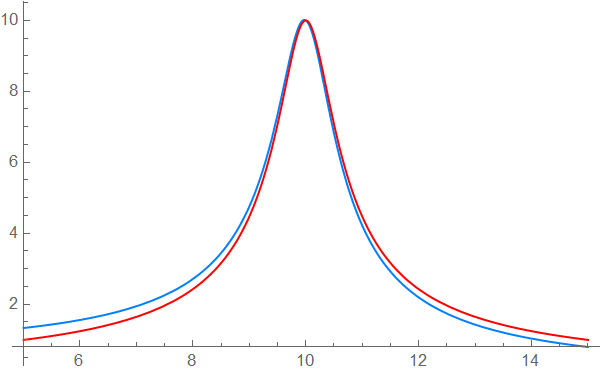
\includegraphics[height = 5cm]{1.png}
    \caption{Plots in Problem 1}
\end{figure}

\paragraph{\large \textbf{Problem 2}}~{\textbf{Solution}}
\vspace{2mm}\\
\noindent (a) Evidently, 
\begin{align}
	\phi &= -\frac{\pi}{4}\\
	b/&m = 4
\end{align}
\par Then
\begin{align}
	\tan \phi = \frac{b\omega_{\text{dr}}}{m(\omega_{\text{dr}}^2-\omega_0^2)}
\end{align}
\par Solving (8)(9)(10), we get
\begin{align}
	\omega_{\text{dr}} = \sqrt{\omega_0^2 + 4} - 2
\end{align}

\noindent (b) Since
\begin{align*}
	A(\Omega_1) &= \frac{F_0}{m\sqrt{(\omega_0^2 - \Omega_1^2)^2 + \left( \frac{b\Omega_1}{m} \right)^2}}\\
	= A(\Omega_2) &= \frac{F_0}{m\sqrt{(\omega_0^2 - \Omega_2^2)^2 + \left( \frac{b\Omega_2}{m} \right)^2}}
\end{align*}
\par we get
\begin{align}
	(\omega_0^2 - \Omega_1^2)^2 + \left( \frac{b\Omega_1}{m} \right)^2 &=(\omega_0^2 - \Omega_2^2)^2 + \left( \frac{b\Omega_2}{m} \right)^2
\end{align}
\par Solving equation(12) we get
\begin{align}
	\omega_0 = \sqrt{(\Omega_1^2 + \Omega_2^2)/2 + \frac{b^2}{m^2}}
\end{align}

\paragraph{\large \textbf{Problem 3}}~{\textbf{Solution}}
\vspace{2mm}
\par In this problem, we set the car as our frame of reference. Suppose the direction of acceleration is pointing to the right.
\par First we consider Problem 2(b) from Problem Set 3. Suppose the magnitude of acceleration is \textit{a}. According to free body diagram(a), we have
\begin{align*}
	\left\{ \begin{array}{l}
		T\cos\theta = mg\\
		T\sin\theta = ma	
	\end{array} \right.
	\quad \Rightarrow \quad
	\theta = \arctan(\frac{a}{g})
\end{align*}
\par Then we consider Problem 2(c) from Problem Set 3. Suppose the mass of the car is \textit{M}. Since the ball is attached to the roof of the car, it shares the same acceleration of that car. Then according to free body diagram(b), for the system we have
\begin{align*}
	\left\{ \begin{array}{l}
		Ma_{\text{car}} = Mg\sin\alpha\\
		a_{\text{car}} = a_{\text{ball}}\\
		ma_{\text{ball}} = mg\sin\theta\\			
	\end{array} \right.	
	\quad \Rightarrow \quad
	\theta = \alpha
\end{align*}
\par Note that all $ma$ in free body diagrams is the force of inertia and others are real forces.
\begin{figure}[H]
    \centering
    \subfigure[Free body diagram of Problem 3.1]{
    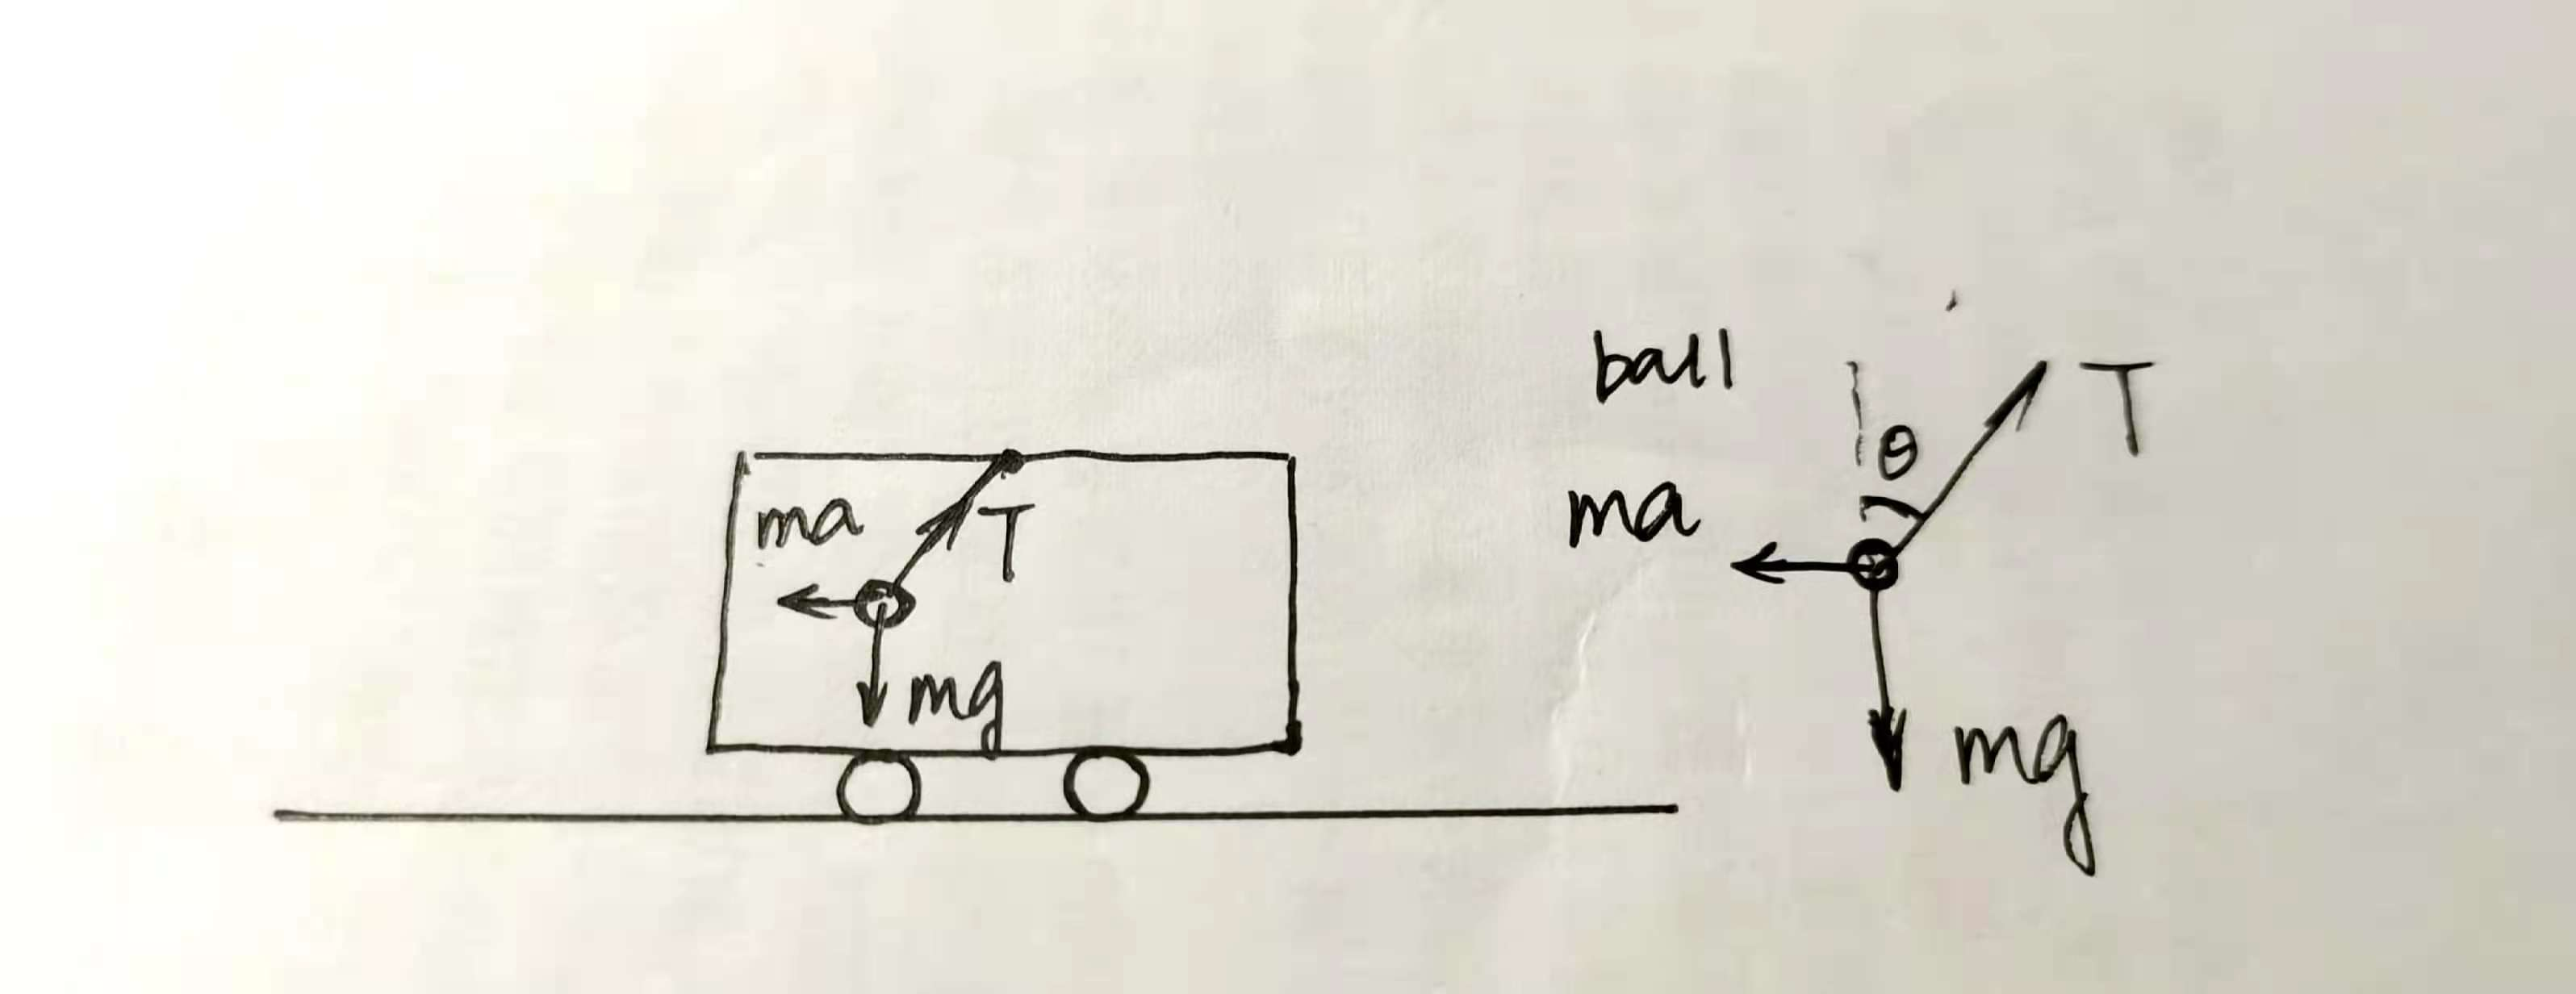
\includegraphics[width = 7.5cm]{1.jpg}
    }
    \subfigure[Free body diagram of Problem 3.2]{
    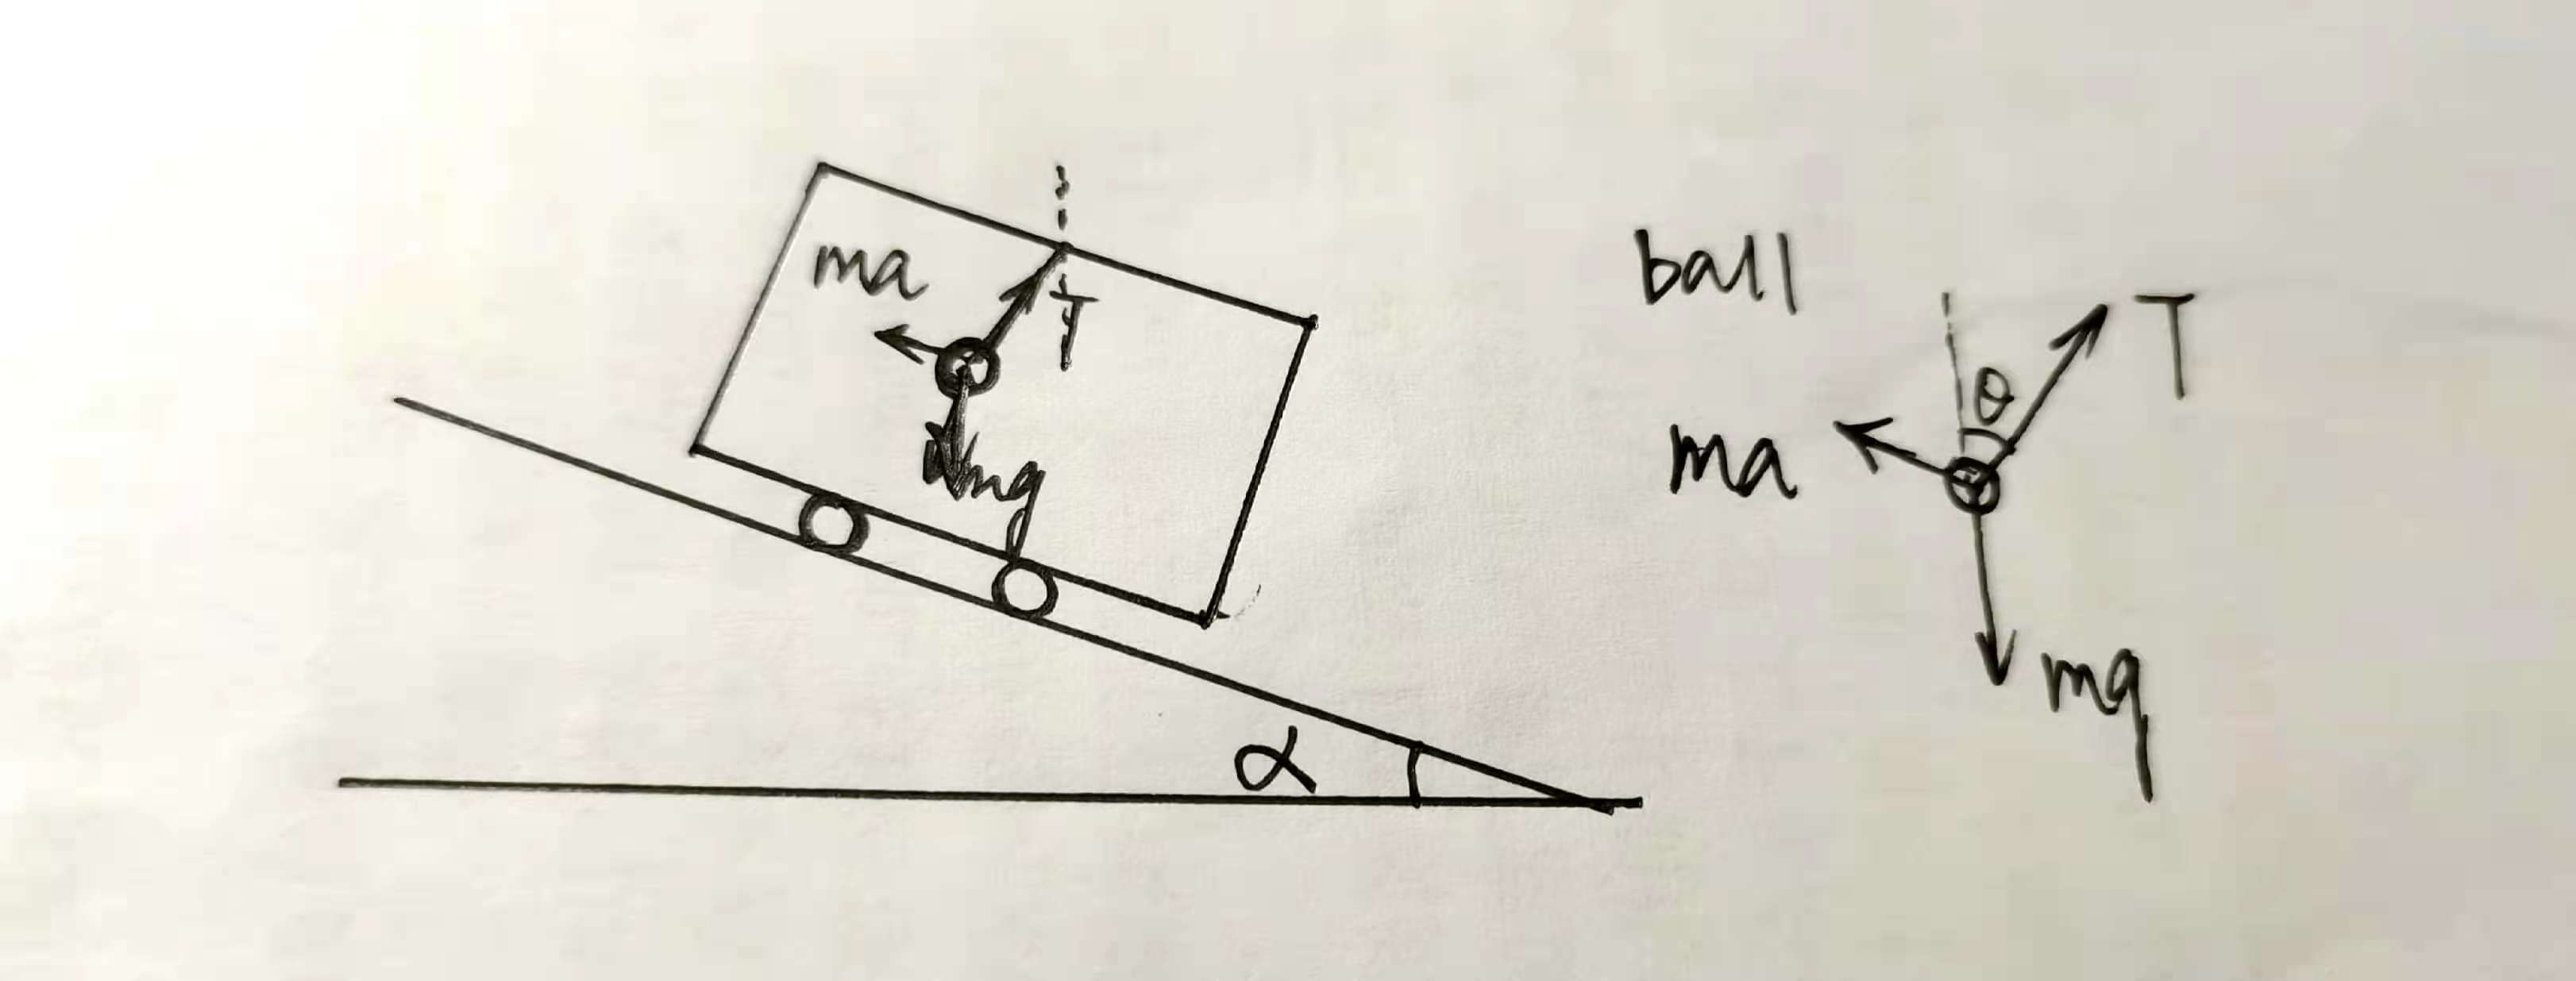
\includegraphics[width = 7.5cm]{2.jpg}
    }
    \caption{Free body diagrams in Problem 3}
\end{figure}

\paragraph{\large \textbf{Problem 4}}~{\textbf{Solution}}
\vspace{2mm}
\par We set the lowerset point fo the parabola as the origin point and denote the coordinate of each point on the parabola by considering the horizontal distance $x$ between itself and the origin point.
\par Apparently this kind of notation cannot determine a point uniquely, however, due to symmetry of parabola, this failure in uniqueness will not affect our purpose to find all the points remaining rest. In addtion,we set the smaller angle between tangential line through the point on the parabola and the horizontal line through the origin point as $\theta$ such that $\tan \theta = \alpha x$.\\
\newline
\noindent (a) According to free body diagram, we have
\begin{align}
	\left\{ \begin{array}{l}
		mg\sin\theta \leq f_{\max}\\
		mg\cos\theta=N\\
		f_{\max}=\mu_sN\\			
	\end{array} \right.	
\end{align}
\par Solving equation system(14) we get
\begin{align}
	x \leq \frac{\mu_s}{\alpha}
\end{align}
\par Therefore, all points whose horizontal distance between the lowest point of the parabola remain at rest if the container is at rest.\\
\newline
\noindent (b) Since the friction has two cases, we will discuss the cases separately.
\par Case 1. The friction is vertical to the support force but directs upwards. According to diagram(c), we know
\begin{align}
	\left\{ \begin{array}{l}
		mg\sin\theta \leq f_{\max}+m\omega^2 x\cos\theta\\
		N=mg\cos\theta+m\omega^2 x\sin\theta\\
		f_{\max}=\mu_s N\\			
	\end{array} \right.	
\end{align}
\par Namely
\begin{align}
	\mu_s\omega^2\alpha\cdot x^2 + (\omega^2-\alpha g)\cdot x +\mu_s g \geq 0
\end{align}


\par Case 2. The friction is vertical to the support force but directs downwards. According to diagram(d), we know
\begin{align}
	\left\{ \begin{array}{l}
		m\omega^2 x\cos\theta \leq f_{\max}+mg\sin\theta\\
		N=mg\cos\theta+m\omega^2 x\sin\theta\\
		f_{\max}=\mu_s N\\			
	\end{array} \right.	
\end{align}
\par Namely
\begin{align}
	\mu_s\omega^2\alpha\cdot x^2 - (\omega^2-\alpha g)\cdot x +\mu_s g \geq 0
\end{align}
\par We then take equation(17)(19) together. Trivially, $x \textgreater 0$. Then we try to solve the inequalities.
\begin{align*}
	\Delta_x &= (\omega^2-g\alpha)^2 - 4(\mu_s g)(\mu_s\omega^2\alpha)\\
	&= \omega^4 - (2g\alpha + 4\mu_s^2\alpha g)\omega^2 + g^2\alpha^2\\
	\Delta_{\omega^2} &= (2g\alpha + 4\mu_s^2\alpha g)^2 - 4g^2\alpha^2\\
	&= 16\mu_s^4g^2\alpha^2 + 16\mu_s^2g^2\alpha^2\\
	\sqrt{\Delta_{\omega^2}} &= 4\mu_s\alpha g \sqrt{\mu_s^2 + 1}\\
	\omega_{1,2}^2 &= \frac{2g\alpha + 4\mu_s^2 g \pm 4\mu_s g\sqrt{\mu_s^2 + 1}}{2}
\end{align*}
\par To make the discussion more clear, we will consider the relative value of $\omega$ and $\alpha g$.
\par From what we know in high scholl, $x_1 + x_2 = -(\omega^2 - \alpha g)/(\mu_s \omega^2\alpha)$ for equation(17) and $x_1 + x_2 = (\omega^2 - \alpha g)/(\mu_s \omega^2\alpha)$ for equation(19). Then we can finally solve equation(17)(19).
\par When $\omega^2 = \frac{2g\alpha + 4\mu_s^2 g - 4\mu_s g\sqrt{\mu_s^2 + 1}}{2} \textless \alpha g$, equation(17) works.
\begin{align*}
	0\ \leq\ x\ \leq\ \frac{\alpha g - \omega^2 - 4\sqrt{\Delta_x}}{2\mu_s\omega^2\alpha}\ \text{or}\ x\ \geq\ \frac{\alpha g - \omega^2 + 4\sqrt{\Delta_x}}{2\mu_s\omega^2\alpha}
\end{align*}
\par When $\omega^2 = \frac{2g\alpha + 4\mu_s^2 g + 4\mu_s g\sqrt{\mu_s^2 + 1}}{2} \textgreater \alpha g$, equation(19) works.
\begin{align*}
	0\ \leq\ x\ \leq\ \frac{\omega^2 - \alpha g - 4\sqrt{\Delta_x}}{2\mu_s\omega^2\alpha}\ \text{or}\ x\ \geq\ \frac{\omega^2 - \alpha g + 4\sqrt{\Delta_x}}{2\mu_s\omega^2\alpha}
\end{align*}
\noindent where $\sqrt{\Delta_x} = \omega^4 - (2g\alpha + 4\mu_s^2\alpha g)\omega^2 + g^2\alpha^2$
\begin{figure}[H]
    \centering
    \subfigure[sketch map of Problem 4]{
    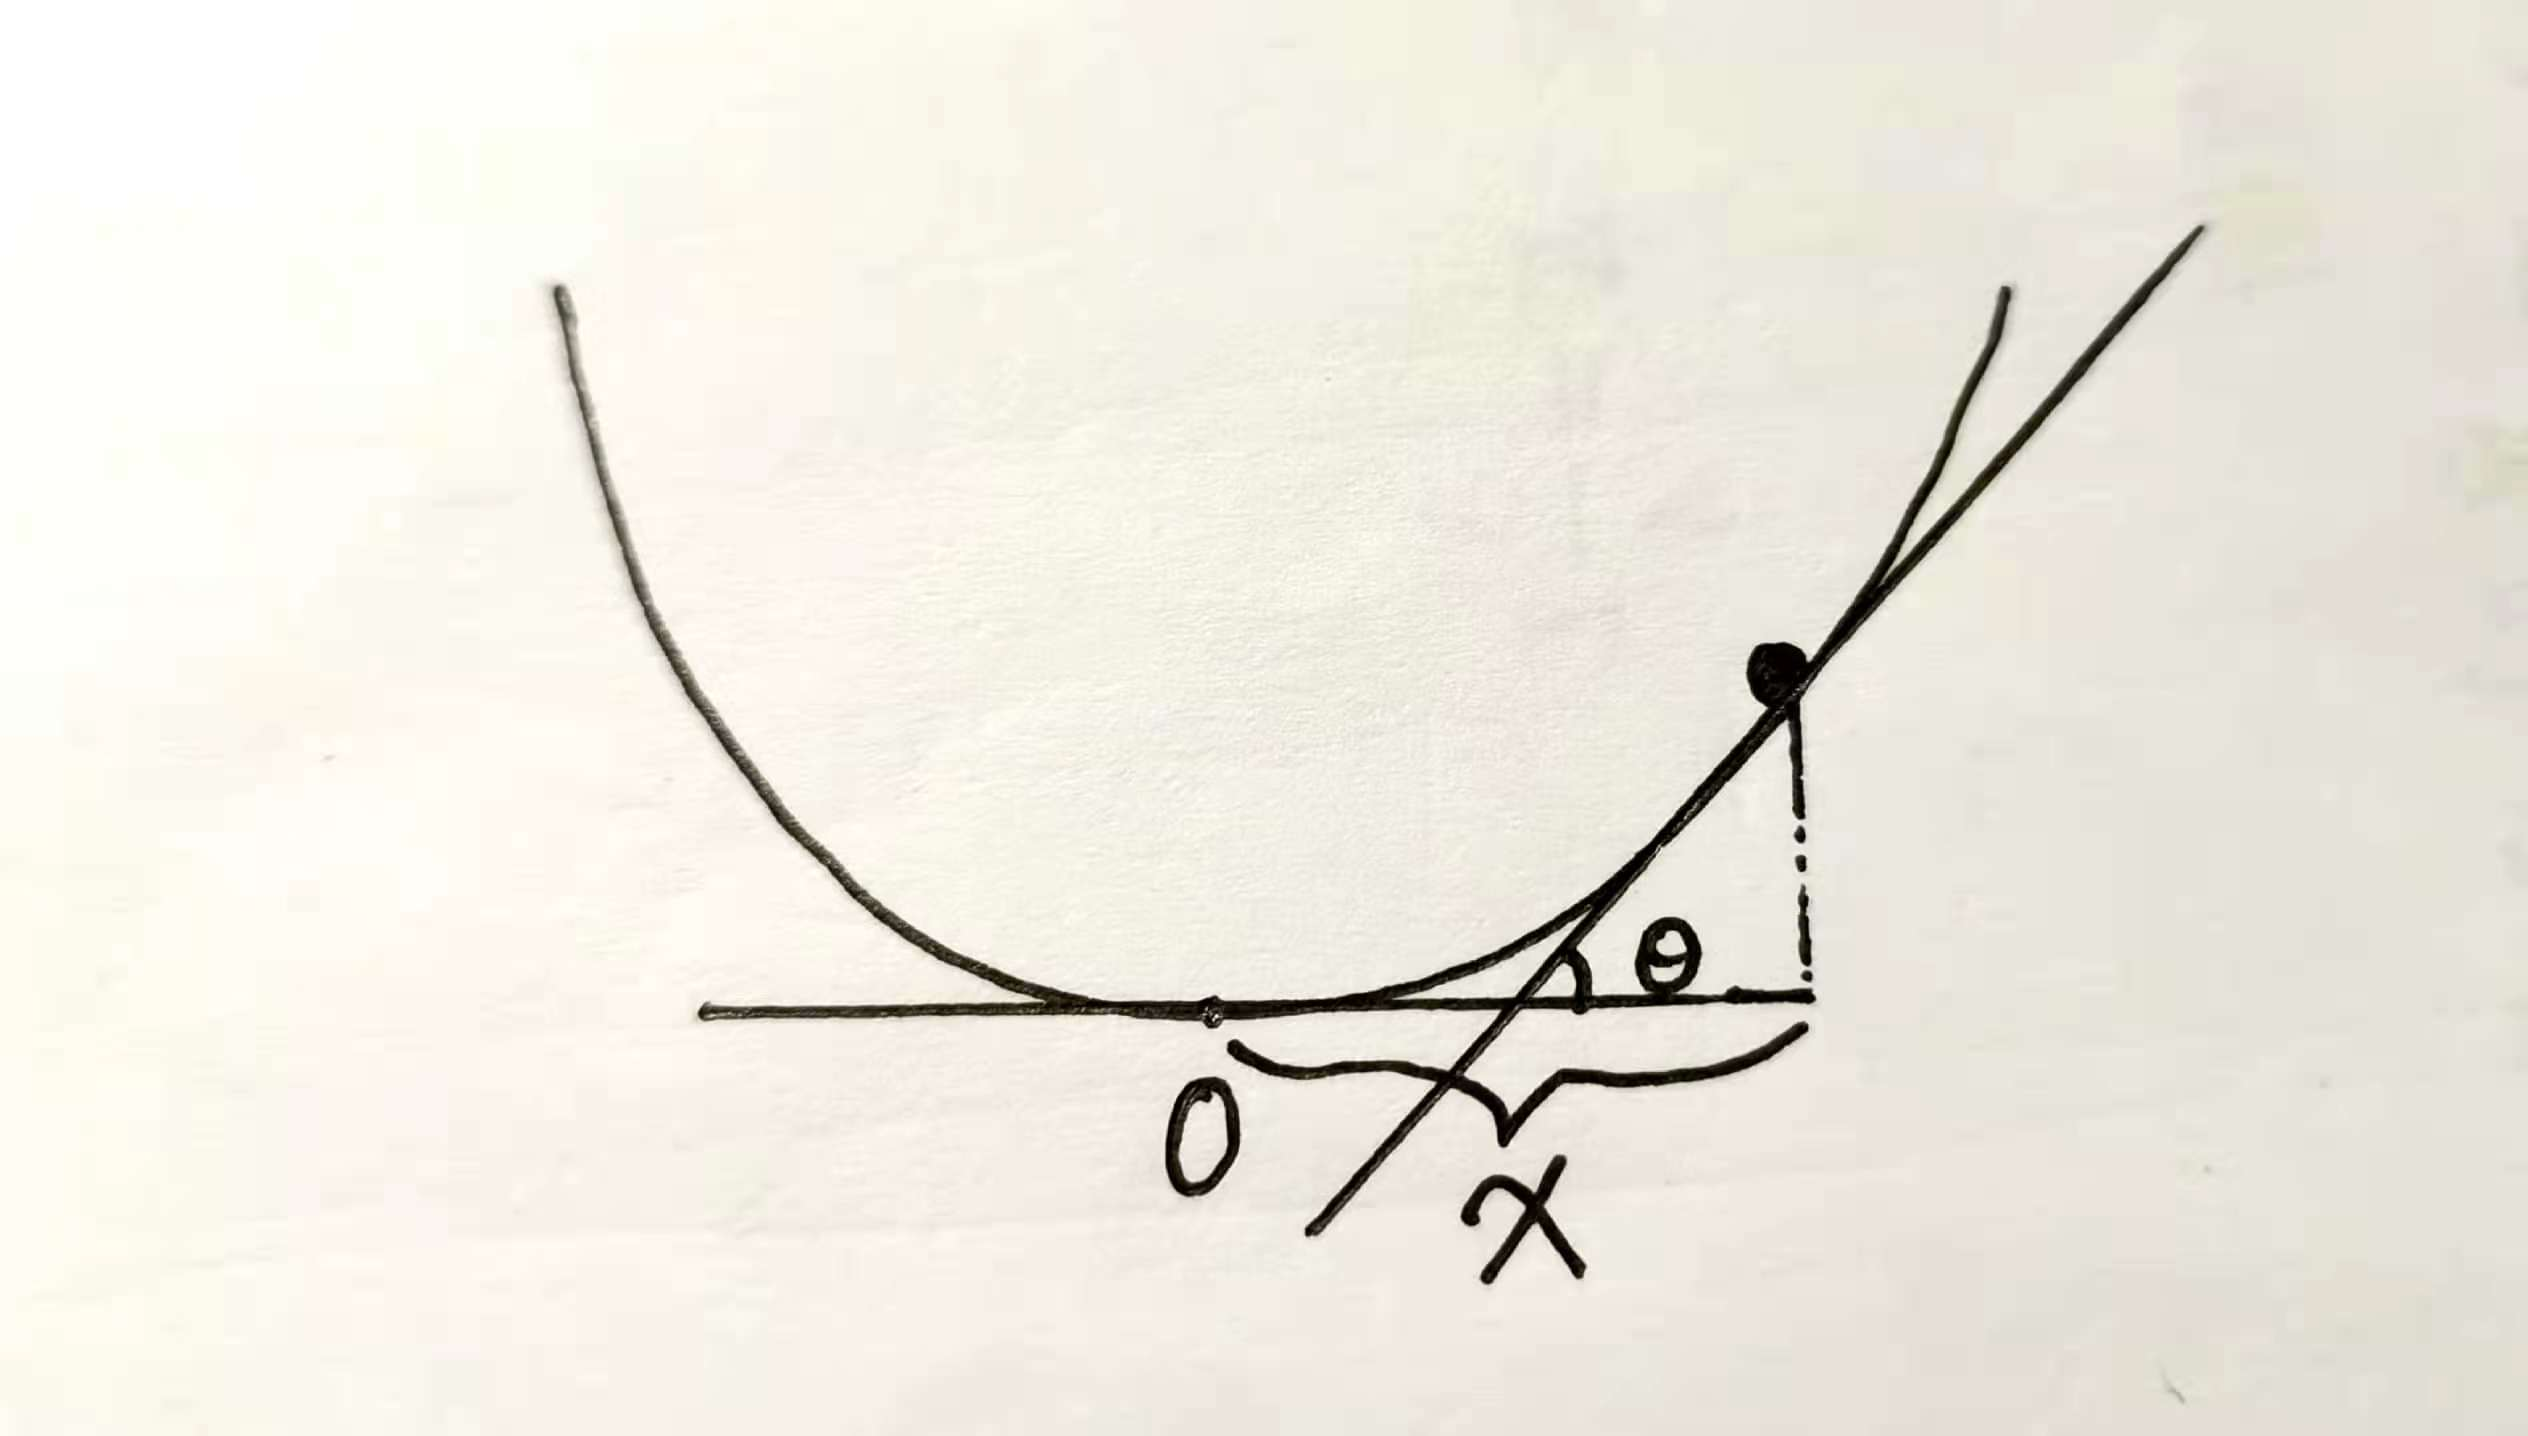
\includegraphics[height = 3cm]{3.jpg}
    }
    \subfigure[free body diagram of Problem4(a)]{
    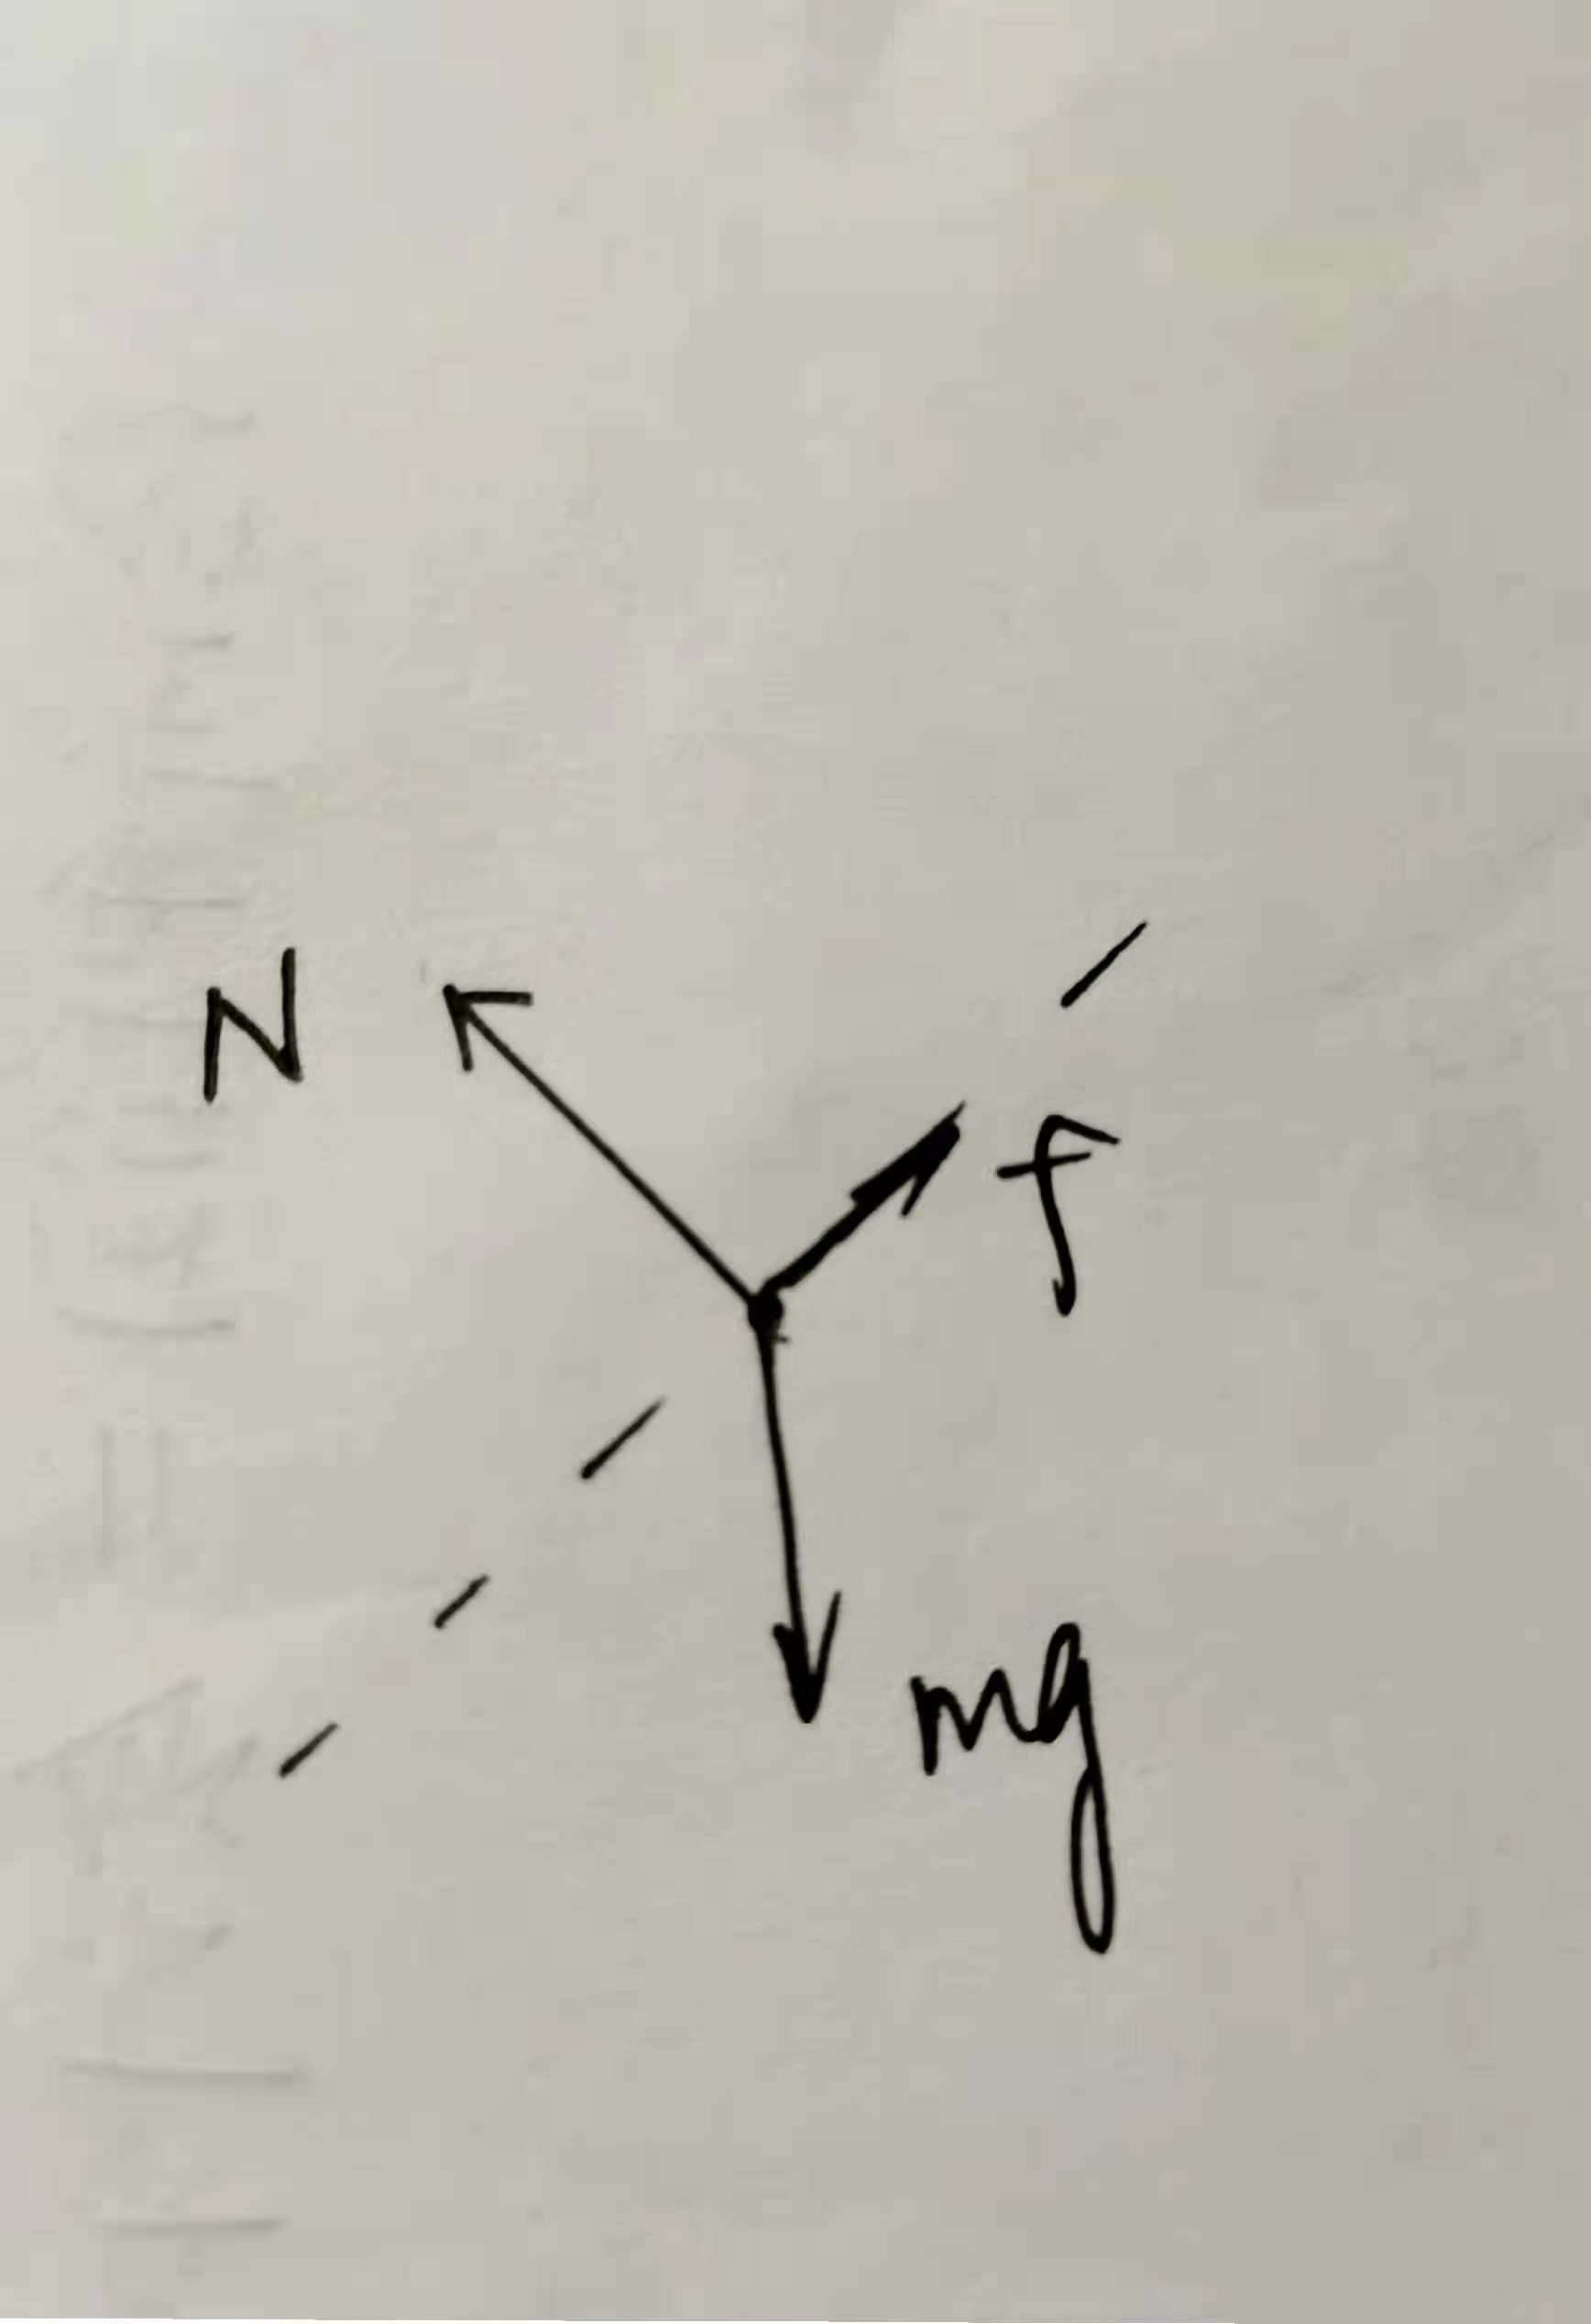
\includegraphics[height = 3cm]{4.jpg}
    }
    \subfigure[free body diagram of Problem4(b) case 1]{
    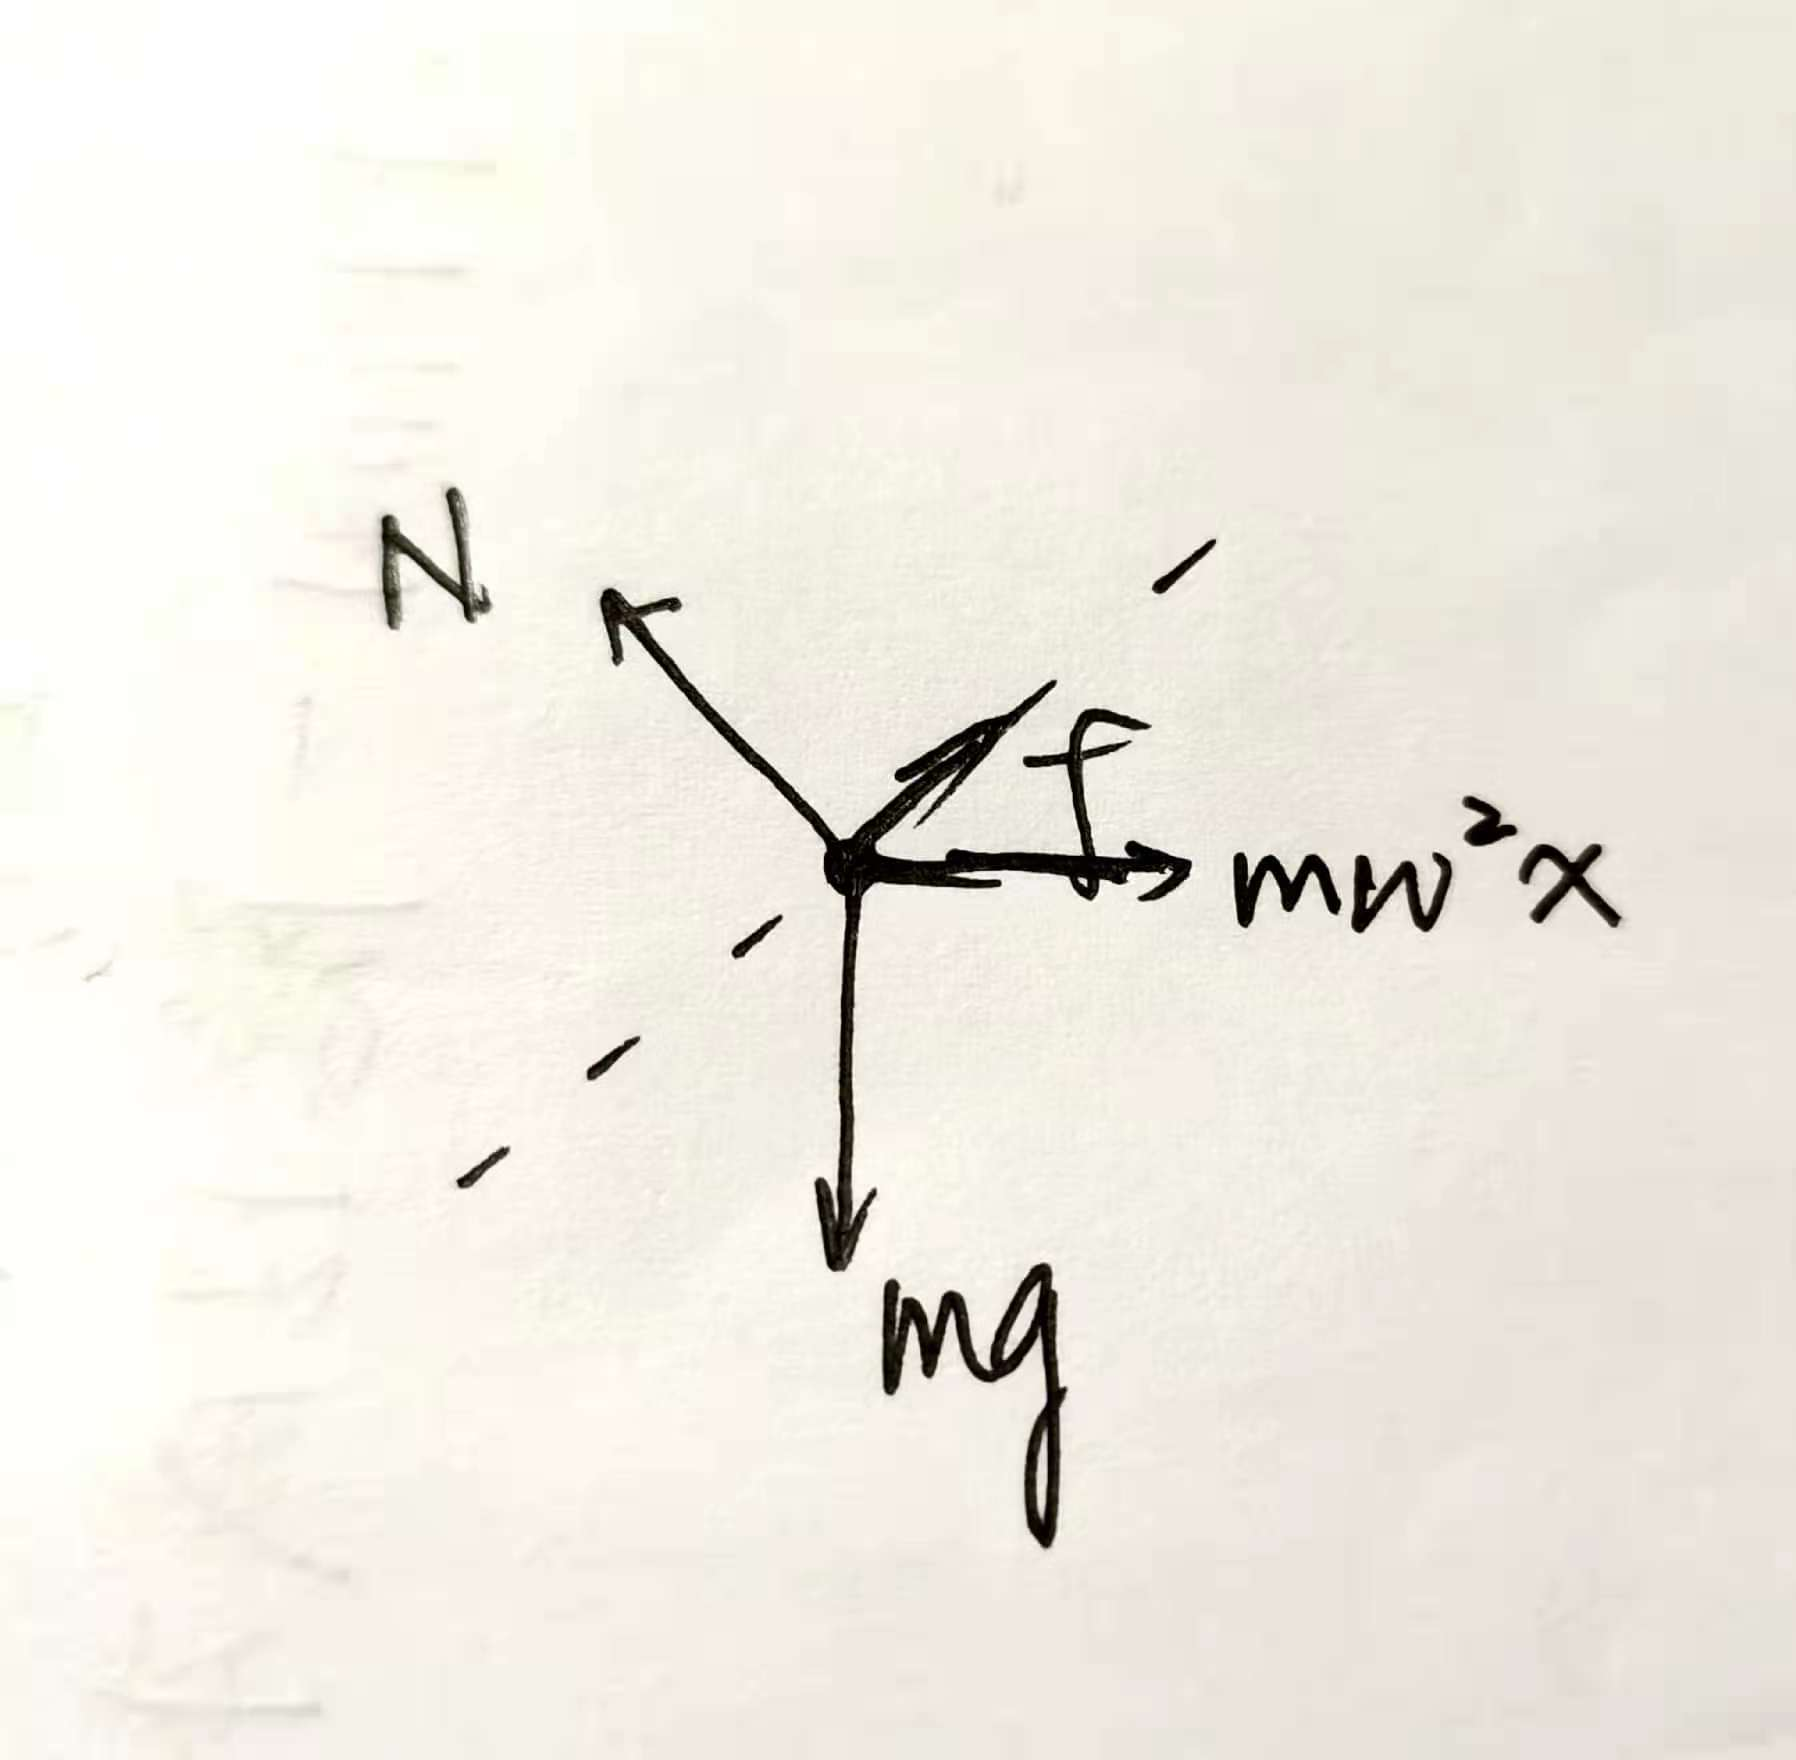
\includegraphics[height = 3cm]{5.jpg}
    }
    \subfigure[free body diagram of Problem4(b) case 2]{
    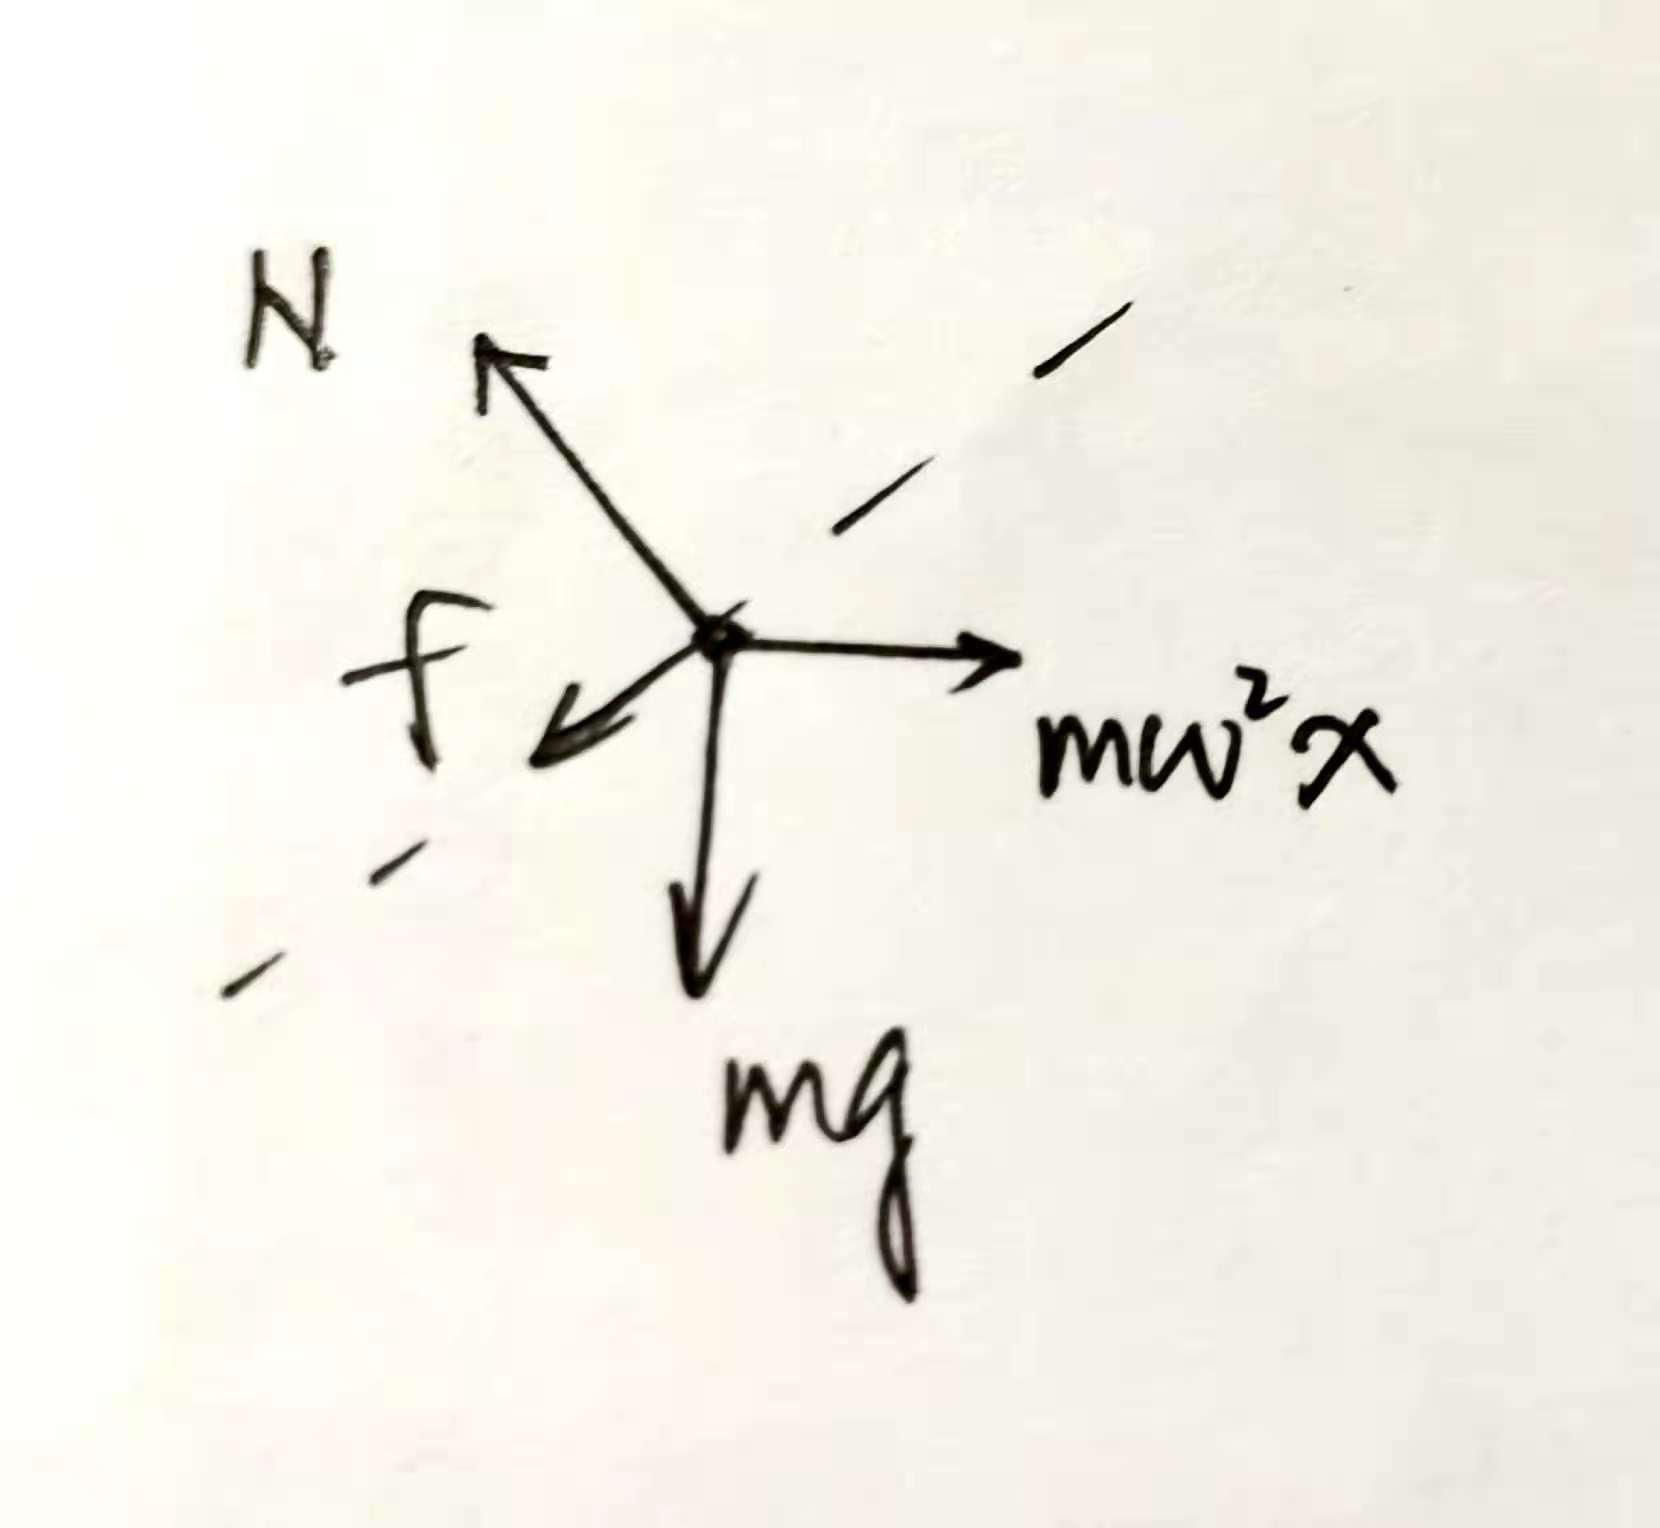
\includegraphics[height = 3cm]{6.jpg}
    }
    \caption{Free body diagrams in Problem 4}
\end{figure}
\paragraph{\large \textbf{Problem 5}}~{\textbf{Solution}}
\vspace{2mm}
\par The direction of the angular acceleration is pointing to the south pole, with no angular accelerations at the poles.
\par The most common phenomenon is release the water in a sink. Before the Earth started to stopp its rotational motion, the person at a pole may see the water current forms a clockwise or counterclockwise swirl while the person on the equator would not see. However, during the Earth stopping its rotational motion, the person at the pole would observe the water current forming a counterclockwise or clockwise swirl corresponding to the previous swirls, however, the one on the equator would observe nothing.

\paragraph{\large \textbf{Problem 6}}~{\textbf{Solution}}
\vspace{2mm}
\par Based on our common sense, they obviously cannot blame their nonproficiency to Coriolis force. We now try to prove this.
\par For the one shooting at a wolf to the west of him, $\langle \omega, v_0 \rangle$ = $90^\circ$ since the west and north is vertical to each other.
\begin{align*}
	\overline{a_c} &= -2 \overline{\omega}\times \overline{v_0}\\
	&= 2\times |\overline{\omega}| \times |\overline{v_0}| \times \sin90^\circ\\
	&= 0.042\ \text{(m/s)}
\end{align*}
\par Then we can calculate the displacement caused by Coriolis force.
\begin{align*}
	\Delta x = \frac{1}{2}a_c t^2 = 0.021\ \text{(m)}
\end{align*}
\par For the one shooting at the wolf to the north of him, $\langle \omega, v_0 \rangle$ = $131^\circ$.
\begin{align*}
	\overline{a_c} &= -2 \overline{\omega}\times \overline{v_0}\\
	&= 2\times |\overline{\omega}| \times |\overline{v_0}| \times \sin131^\circ\\
	&= 0.032\ \text{(m/s)}
\end{align*}
\par Then we can calculate the displacement caused by Coriolis force.
\begin{align*}
	\Delta x = \frac{1}{2}a_c t^2 = 0.016\ \text{(m)}
\end{align*}
\end{document}